\documentclass[tikz,border=3mm,multi=tikzpicture]{standalone}
\usepackage[utf8]{inputenc}
\usepackage[T1]{fontenc}
\usepackage{helvet}
\renewcommand{\familydefault}{\sfdefault}
\usepackage{tikz}
\usetikzlibrary{angles,quotes,calc,intersections}
\begin{document}

\tikzset{every node/.append style={font=\sffamily\small}}
% TikZ 1
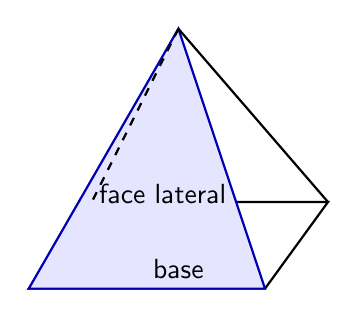
\begin{tikzpicture}[scale=1]
\coordinate (A) at (0,0); \coordinate (B) at (3,0); \coordinate (C) at (3.8,1.1); \coordinate (D) at (.8,1.1); \coordinate (V) at (1.9,3.3);
\draw[thick] (A)--(B)--(C)--(D)--cycle;
\draw[fill=blue!10,draw=blue!70!black,thick] (V)--(A)--(B)--cycle;
\draw[thick] (V)--(C); \draw[thick,dashed] (V)--(D);
\node at (1.9,.25) {base};
\node at (1.7,1.2) {face lateral};
\end{tikzpicture}
% TikZ 2
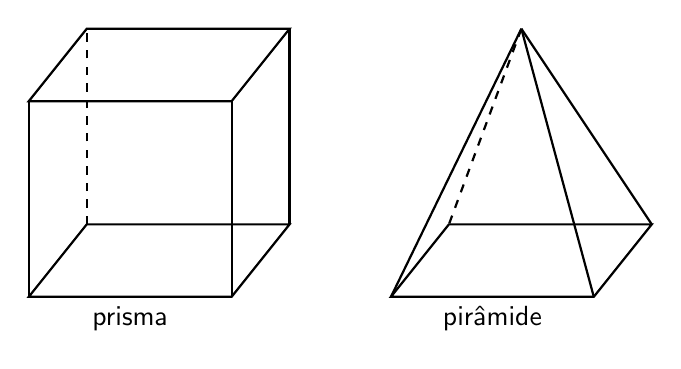
\begin{tikzpicture}[scale=.92]
\coordinate (A) at (0,0); \coordinate (B) at (2.8,0); \coordinate (C) at (3.6,1); \coordinate (D) at (.8,1);
\coordinate (E) at (0,2.7); \coordinate (F) at (2.8,2.7); \coordinate (G) at (3.6,3.7); \coordinate (H) at (.8,3.7);
\draw[thick] (A)--(B)--(C)--(D)--cycle; \draw[thick] (E)--(F)--(G)--(H)--cycle;
\draw[thick] (A)--(E); \draw[thick] (B)--(F); \draw[thick] (C)--(G); \draw[thick,dashed] (D)--(H);
\node[below] at (1.4,0) {prisma};
\coordinate (I) at (5,0); \coordinate (J) at (7.8,0); \coordinate (K) at (8.6,1); \coordinate (L) at (5.8,1); \coordinate (V) at (6.8,3.7);
\draw[thick] (I)--(J)--(K)--(L)--cycle; \draw[thick] (V)--(I); \draw[thick] (V)--(J); \draw[thick] (V)--(K); \draw[thick,dashed] (V)--(L);
\node[below] at (6.4,0) {pirâmide};
\end{tikzpicture}


% TikZ 3
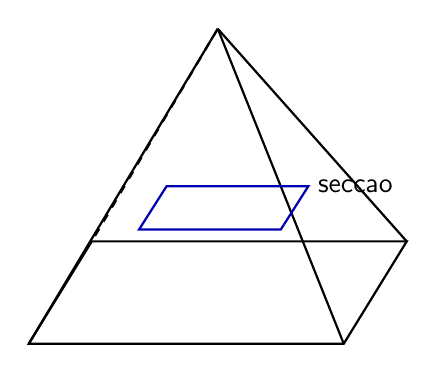
\begin{tikzpicture}[scale=1]
\coordinate (A) at (0,0); \coordinate (B) at (4,0); \coordinate (C) at (4.8,1.3); \coordinate (D) at (.8,1.3); \coordinate (V) at (2.4,4);
\coordinate (A2) at (1.4,1.45); \coordinate (B2) at (3.2,1.45); \coordinate (C2) at (3.55,2.0); \coordinate (D2) at (1.75,2.0);
\draw[thick] (A)--(B)--(C)--(D)--cycle;
\draw[thick] (V)--(A); \draw[thick] (V)--(B); \draw[thick] (V)--(C); \draw[thick,dashed] (V)--(D);
\draw[blue!70!black,thick] (A2)--(B2)--(C2)--(D2)--cycle;
\node[right] at (C2) {seccao};
\end{tikzpicture}
% TikZ 4
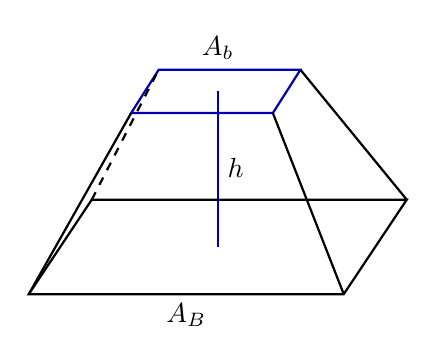
\begin{tikzpicture}[scale=1]
\coordinate (A) at (0,0); \coordinate (B) at (4,0); \coordinate (C) at (4.8,1.2); \coordinate (D) at (.8,1.2);
\coordinate (E) at (1.3,2.3); \coordinate (F) at (3.1,2.3); \coordinate (G) at (3.45,2.85); \coordinate (H) at (1.65,2.85);
\draw[thick] (A)--(B)--(C)--(D)--cycle;
\draw[thick,blue!70!black] (E)--(F)--(G)--(H)--cycle;
\draw[thick] (A)--(E); \draw[thick] (B)--(F); \draw[thick] (C)--(G); \draw[thick,dashed] (D)--(H);
\draw[blue!70!black,thick] (2.4,.6)--(2.4,2.58);
\node[right] at (2.4,1.6) {$h$};
\node[below] at (2,0) {$A_B$};
\node[above] at (2.4,2.85) {$A_b$};
\end{tikzpicture}
\end{document}
